\documentclass[a4paper, twocolumn]{article}
\usepackage[pdftex, hidelinks]{hyperref}

\usepackage{bm}
\usepackage[T1]{fontenc}
\usepackage[utf8]{inputenc}
\usepackage{algpseudocode}
\usepackage{algorithm}
\usepackage{amsfonts}
\usepackage{amssymb}
\usepackage{courier}
\usepackage{booktabs}
\usepackage{graphicx}
\usepackage{listings}
\usepackage{mathtools}
\usepackage{amssymb}
\lstset{basicstyle=\footnotesize\ttfamily,
        breakatwhitespace = false,
        breaklines = true,
        keepspaces = true,
        language = R,
        showspaces = false,
        showstringspaces = false,
        belowcaptionskip = \bigskipamount,
        framerule = 0.80pt,
        frame = tb,
        belowskip = \bigskipamount,
        escapeinside={<@}{@>}}

\title{TDDE01 -- Machine Learning \\
       Group 9 Laboration Report 1}
\author{{Martin Estgren \texttt{<mares480>}} \\
        {Björn Jansson \texttt{<bjoja408>}} \\
        {Erik S. V. Jansson \texttt{<erija578>}} \\
        {Sebastian Maghsoudi \texttt{<sebma654>}} \\~\\
        {Linköping University (LiU), Sweden}}

\begin{document}
    \pagenumbering{arabic}
    \maketitle % Generate.

    \section*{Assignment 1}

    Nobody likes \emph{e-mail spam}, therefore methods for autonomously \emph{predicting} if a given e-mail is probably \emph{spam} or \emph{not spam} is an important task. This is a classic example where \emph{machine learning} is useful; given a set of \emph{training data} and \emph{testing data}, can we predict what is \emph{spam} and \emph{not spam} in the \emph{testing set} (without knowing the answer) by deriving a \emph{hypothesis function} built from the \emph{training data}?

    By using \emph{k-nearest neighbor classification}, one can derive if an e-mail is spam or not by simply looking at \emph{similar e-mails/messages}, and picking the most likely solution by doing a \emph{``majority vote''}. First, a \emph{distance function} needs to be implemented, which is the \emph{cosine distance function} in Equation~\ref{eq:distance}, whose implementation can be found in Listing~\ref{lst:distance}, but with a optimized solution using only matrices.

    \begin{equation} \label{eq:distance}
        d(X,Y) = 1 - \frac{X^TY}{\sqrt{\sum_i{X_i^2}}\sqrt{\sum_i{Y_i^2}}}
    \end{equation}

    After defining the distance function $d(X,Y)$, one can find the \emph{e-mail/message distance} for each $Y_j$ in respect to each $X_i$. Where $X$ is the \emph{testing set} and $Y$ the \emph{training set}. Each row of the resulting matrix contains the relative distance between $X_i$ and $\forall Y_j$. Therefore, sorting each row $X_i$ and picking the first $K$ elements gives the $K$ \emph{closest messages} from the \emph{training set} in respect to each \emph{testing element}. By using this, the \emph{k-nearest neighbors} can be found, and the prediction of $\hat{Y}$ (spam, not spam) is done by using Equation~\ref{eq:knn}, where $K_i$ classify as being $C_i$.

    \begin{equation} \label{eq:knn}
        \hat{Y} = \underset{\forall C_i}{\mathrm{max}}\; p(C_i | \bm{x}),\; p(C_i | \bm{x}) \propto K_i \div K
    \end{equation}

    The \emph{k-nearest neighbor algorithm} is implemented in Listing~\ref{lst:knearest}, in the function \texttt{knearest(t,k,t')}. It works as previously described, where line \texttt{20} is calculating the \emph{distance matrix} and line \texttt{21} sorting each row, so that all $Y$ distances are relative to $X_i$. Thereafter, in line \texttt{26-27} the classification is found for the $K$-nearest neighbors of $X_i$. The \emph{mean} value is then taken, which is equivalent to $K_i \div K$ since only two classifications exist (spam and not spam), following a \emph{Cover et al.}~\cite{cover1967nearest} K-NN descriptions.

    From the \textit{knearest} function we get a vector containing all the predicted classifications for the data set. First we set a probability threshold \( p(\mathbf{x} |\theta) > 0.5\) and compare the predicted classifications with the true classifications in the data set. Where the threshholds are done in lines \texttt{49-50} in the main spam classification script found under a Listing~\ref{lst:spam}.

    The result for \(k = 5,\, k = 1\) can be observed in the following tables, for both \emph{kknn} and \emph{knearest.r}:
\begin{verbatim}
            knearest, k = 5
observations   0   1
           0 682 263
           1 186 239
misclassification rate = 0.3277372
\end{verbatim}
    These results indicate a ``hit ratio'' of around \(68 \%\).

\begin{verbatim}
            knearest, k = 1
observations   0   1
           0 650 295
           1 174 251
misclassification rate = 0.3423358
\end{verbatim}
    These results indicate a ``hit ratio'' of around \(66 \%\) for the results when \emph{knearest} has $k=1$ neighbors.

    The result indicates that our classifier is fairly good for the given data set but to get a better perspective we compare it to a built in classifier called \textit{Weighted K-nearest neighbor} (kknn) on the same training and testing data set. The result can be observed bellow,\, for both $k=1$ and $k=5$ values:

\begin{verbatim}
            kknn, k = 5, k = 1
observations   0   1
           0 626 319
           1 184 241
misclassification rate = 0.3671533
\end{verbatim}
    The biggest difference from out own implementation is that the hit rate and confusion matrix are identical for both \(K = 1\) and \(K = 5\). The hit rate is also slightly lower that ours at about \( 0.63\).

    We then proceed to plot the classifiers in a \textit{ROC - curve} for the probability threshold \( p(x) > 0.05,...,0.95\) with steps of \(0.01\). Where the \emph{x-axis} shows the \emph{sensitivity}/\emph{true positive rate} and the \emph{y-axis} shows the \emph{false negative rate}. 
The \textit{true positive rate} is calculated as
\begin{equation}
 \frac{Tp}{Tp + Fn}
\end{equation}
where \(Tp\) stands for the \textit{true positives} i.e. the cases where both the prediction and observations classified the case as \textit{true}, and \(Fn\) stands for the \textit{false negatives} i.e. the cases where the prediction was \textit{false} but the observation was \textit{true}.

The \textit{true negative rate} is calculated as \(1 - specificity\) where \textit{specificity} is equal to:
\begin{equation}
 \frac{Tn}{Tn + Fp}
\end{equation}
where \(Tn\) stands for the \textit{true negatives} i.e. the cases where both the prediction and observations classified the case as \textit{false}, and \(Fp\) stands for the \textit{false positives} i.e. the cases where the prediction was \textit{true} but the observation was \textit{false}.

These operations can be found in the lines \texttt{95-97} for \emph{knearest} and \texttt{109-111} for \emph{kknn} in Listing~\ref{lst:spam} \texttt{spam.r}.

    The resulting \textit{ROC - curve} can be observed in the column to the right, that is in the Figure~\ref{fig:roc}.

    Blue curve is \textit{knearest} and green curve is \textit{kknn}. The red line is a reference line for a random classifier. The result indicates as with the confusion matrices that our \textit{knearest} implementation slightly out performs \textit{kknn} on some threshold variables.

\begin{figure}[H]
\centering
\begin{minipage}[]{0.5\textwidth}
  \includegraphics[width=\textwidth]{share/Lab1_A1_ROC.png}  
  \caption{ROC - curve of  \textit{knearest} and  \textit{kknn}.\label{fig:roc} }
 \end{minipage}
\end{figure}

    \section*{Assignment 2}

	The first part of the assignment was completed by importing the data from a csv-file and assuming that the probability is exponentially distributed. Because \(L(\theta | x) = p(\theta|x)\)  [1], one can derive the log-likelihood in the following steps:\newline
	
	{\large \(L(\theta | x) = {\displaystyle \prod_{i = 0}^{n}}p(x_i|\theta) \newline = \displaystyle \prod_{i = 0}^{n}\theta e^{-\theta x}=\theta^n exp(-\theta \sum_{i=0}^{n}x_i) \newline \implies ln L(\theta | x)) = n ln(\theta) - \theta \sum_{i=0}^n x_i \)}
	\newline
	
	Having this formulae, the sum of observations is constant as well as the length (n) of the data. Thus, one can simply plot the return value of the function for all reasonable values (0.05-4) for \(\theta\). In order to use the maximum-likelihood method to estimate \(\theta\), one simply picks the theta that is most likely to produce the observed data i.e. the \(\theta\) that produced the highest value of \(ln( L(\theta | x))\). In order to investigate how the size of the observed data affect the estimation of \(\theta\), one might simply use less of the data. \newline\newline
	The posterior probability[2] is also called the reverse probability i.e. \(p(\theta|x)\) meaning the probability for \(\theta\) given observed data \(x\).This can be calculated in this context with \(p(x|\theta)p(\theta)\) where \(p(\theta)\) is given in the assignment description as \(10 e^{-10\theta }\). Also here the ln version of the functions may be used since the functionality is already defined earlier. This would not change the estimation of the optimal \(\theta\) since the maximum value for ln(f(x)) and f(x) dosn't change [1]. In order to use already defined functions, one can make the following derivations:\newline
	
	{\large \(ln(p(x|\theta)p(\theta)) = ln L\theta|x)p(\theta)) \newline = ln L) + ln(p(\theta))\)} \newline
	
	In order to find the most optimal estimation of \(\theta\) one simply elects the theta that produces the highest value of said function.
	
	Given that we use all the data and apply said data on said log-likelihood function previously described, the output is persented in figure \ref{fig:likelihood}. The maximum likelihood method gives us an estimation of \(\theta = 1.1262\). When using less of the data we produce another value \(\theta = 1.7857\) however as can be seen in figure \ref{fig:likelihood}, on the blue curve most values are not significantly different from the maximum value. This means one can not be certain when estimating \(\theta\) since other options are also viable. The black curve in figure \ref{fig:likelihood}, the estimated \(\theta \)
	
	\begin{figure}[H]
		\centering
		\begin{minipage}[]{0.5\textwidth}
			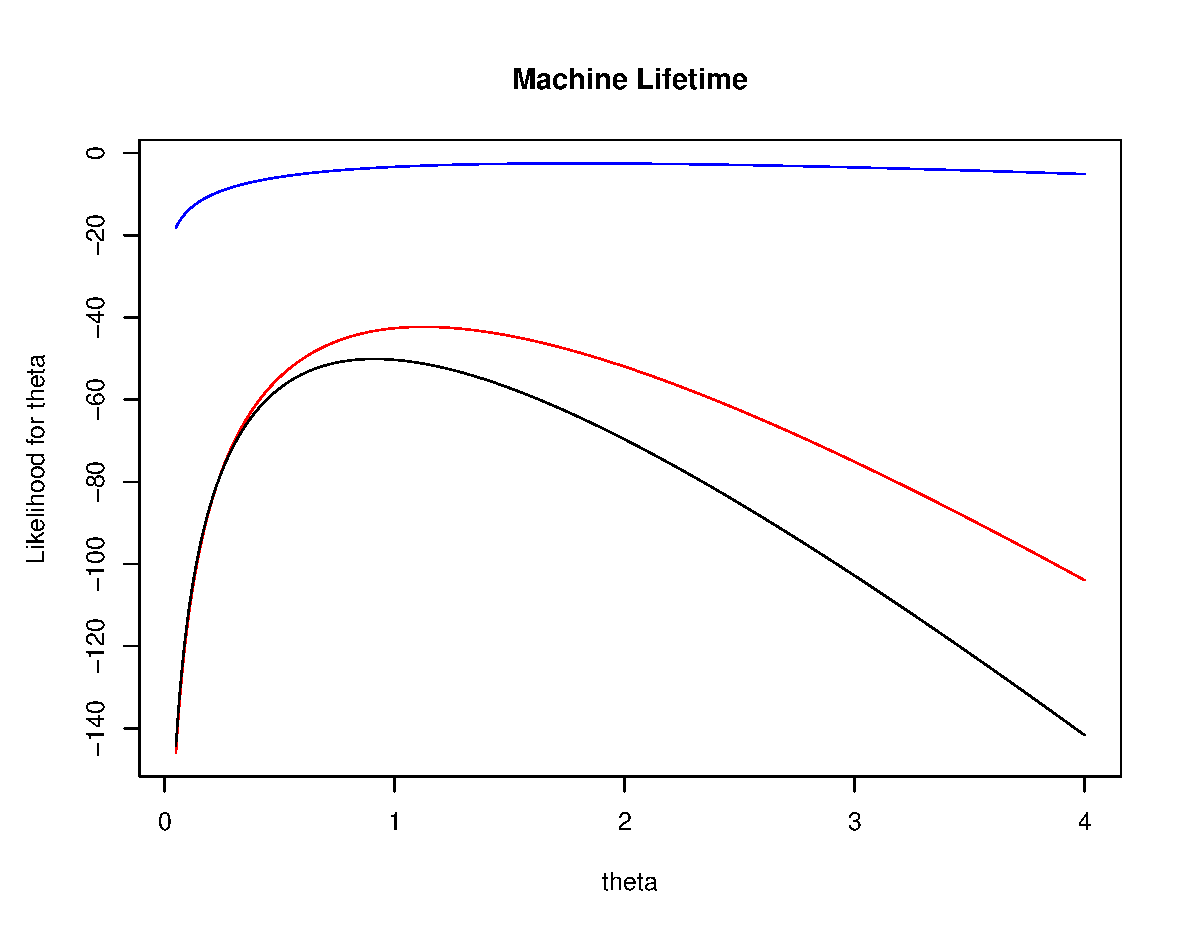
\includegraphics[width=\textwidth]{share/loglike.eps}  
			\caption{Log-likelihood \& postiori curves.\label{fig:likelihood} }
		\end{minipage}
	\end{figure}
	
	 The presentation of the distribution of the observed data can be viewed in figure \ref{fig:hist}, in the left histogram. The right histogram however, a randomly generated data set of 50 values is generated. The data is not completely random, but generated using an exponential distribution given the \(theta\) estimated from the 48 given data values. This of course would imply that the data sets look similar when plotted in a histogram. However this does not necessarily imply that they are representative of the entire population since the posterori-probability was neglected for this measure. 

\begin{figure*}[h]
	\includegraphics[width=0.5\textwidth]{share/hist_original.eps}
	\includegraphics[width=0.5\textwidth]{share/hist_rexp.eps}
	\caption{\label{fig:hist}Histogram for original and generated data.}
\end{figure*}

    \section*{Contributions}

    \begin{itemize}
        \item{\textbf{Erik S. V. Jansson:} wrote the initial section in \emph{Assignment 1} regarding on how the \emph{k-nearest neighbor algorithm} works, and also provided the \texttt{knearest} scripts in Listings~\ref{lst:knearest},\ref{lst:distance}.}
        \item{\textbf{Martin Estgren:} wrote the sections on generating \emph{confusion matrices} and the \emph{missclassification ratio} of \emph{knearest} and \emph{kknn}. Additionally, on how to generate \emph{ROC-curves} and the plot itself. Finally, he provided Listing~\ref{lst:spam} which wraps the script functions in assignment 1 up. Additionally, he also extended the formula description on \emph{ROC-curves} for full completeness.}
        \item{\textbf{Bjorn Jansson:} Wrote the third section.}
        \item{\textbf{Sebastian Maghsoudi:} Wrote the first, second and fourth section.}
    \end{itemize}

    \nocite{*} % No warnings.
    \bibliographystyle{alpha}
    \bibliography{report}
    \onecolumn \appendix
    \section*{Appendix}

    \lstinputlisting[caption={K-Nearest Neighbor Algorithm Implementation},label={lst:knearest}]{share/knearest.r}
    \lstinputlisting[caption={Cosine Cost/Distance Formula},label={lst:distance}]{share/distance.r}
    \lstinputlisting[caption={Main Spam Prediction Script},label={lst:spam}]{share/spam.r}

\end{document}
